\documentclass[11pt,]{article}
\usepackage{lmodern}
\usepackage{amssymb,amsmath}
\usepackage{ifxetex,ifluatex}
\usepackage{fixltx2e} % provides \textsubscript
\ifnum 0\ifxetex 1\fi\ifluatex 1\fi=0 % if pdftex
  \usepackage[T1]{fontenc}
  \usepackage[utf8]{inputenc}
\else % if luatex or xelatex
  \ifxetex
    \usepackage{mathspec}
  \else
    \usepackage{fontspec}
  \fi
  \defaultfontfeatures{Ligatures=TeX,Scale=MatchLowercase}
\fi
% use upquote if available, for straight quotes in verbatim environments
\IfFileExists{upquote.sty}{\usepackage{upquote}}{}
% use microtype if available
\IfFileExists{microtype.sty}{%
\usepackage{microtype}
\UseMicrotypeSet[protrusion]{basicmath} % disable protrusion for tt fonts
}{}
\usepackage[margin = 1.5in]{geometry}
\usepackage{hyperref}
\PassOptionsToPackage{usenames,dvipsnames}{color} % color is loaded by hyperref
\hypersetup{unicode=true,
            pdftitle={Introduction to Data Reading and Tidying},
            pdfauthor={Abhinav Anand, IIMB},
            colorlinks=true,
            linkcolor=blue,
            citecolor=magenta,
            urlcolor=red,
            breaklinks=true}
\urlstyle{same}  % don't use monospace font for urls
\usepackage{color}
\usepackage{fancyvrb}
\newcommand{\VerbBar}{|}
\newcommand{\VERB}{\Verb[commandchars=\\\{\}]}
\DefineVerbatimEnvironment{Highlighting}{Verbatim}{commandchars=\\\{\}}
% Add ',fontsize=\small' for more characters per line
\usepackage{framed}
\definecolor{shadecolor}{RGB}{248,248,248}
\newenvironment{Shaded}{\begin{snugshade}}{\end{snugshade}}
\newcommand{\KeywordTok}[1]{\textcolor[rgb]{0.13,0.29,0.53}{\textbf{#1}}}
\newcommand{\DataTypeTok}[1]{\textcolor[rgb]{0.13,0.29,0.53}{#1}}
\newcommand{\DecValTok}[1]{\textcolor[rgb]{0.00,0.00,0.81}{#1}}
\newcommand{\BaseNTok}[1]{\textcolor[rgb]{0.00,0.00,0.81}{#1}}
\newcommand{\FloatTok}[1]{\textcolor[rgb]{0.00,0.00,0.81}{#1}}
\newcommand{\ConstantTok}[1]{\textcolor[rgb]{0.00,0.00,0.00}{#1}}
\newcommand{\CharTok}[1]{\textcolor[rgb]{0.31,0.60,0.02}{#1}}
\newcommand{\SpecialCharTok}[1]{\textcolor[rgb]{0.00,0.00,0.00}{#1}}
\newcommand{\StringTok}[1]{\textcolor[rgb]{0.31,0.60,0.02}{#1}}
\newcommand{\VerbatimStringTok}[1]{\textcolor[rgb]{0.31,0.60,0.02}{#1}}
\newcommand{\SpecialStringTok}[1]{\textcolor[rgb]{0.31,0.60,0.02}{#1}}
\newcommand{\ImportTok}[1]{#1}
\newcommand{\CommentTok}[1]{\textcolor[rgb]{0.56,0.35,0.01}{\textit{#1}}}
\newcommand{\DocumentationTok}[1]{\textcolor[rgb]{0.56,0.35,0.01}{\textbf{\textit{#1}}}}
\newcommand{\AnnotationTok}[1]{\textcolor[rgb]{0.56,0.35,0.01}{\textbf{\textit{#1}}}}
\newcommand{\CommentVarTok}[1]{\textcolor[rgb]{0.56,0.35,0.01}{\textbf{\textit{#1}}}}
\newcommand{\OtherTok}[1]{\textcolor[rgb]{0.56,0.35,0.01}{#1}}
\newcommand{\FunctionTok}[1]{\textcolor[rgb]{0.00,0.00,0.00}{#1}}
\newcommand{\VariableTok}[1]{\textcolor[rgb]{0.00,0.00,0.00}{#1}}
\newcommand{\ControlFlowTok}[1]{\textcolor[rgb]{0.13,0.29,0.53}{\textbf{#1}}}
\newcommand{\OperatorTok}[1]{\textcolor[rgb]{0.81,0.36,0.00}{\textbf{#1}}}
\newcommand{\BuiltInTok}[1]{#1}
\newcommand{\ExtensionTok}[1]{#1}
\newcommand{\PreprocessorTok}[1]{\textcolor[rgb]{0.56,0.35,0.01}{\textit{#1}}}
\newcommand{\AttributeTok}[1]{\textcolor[rgb]{0.77,0.63,0.00}{#1}}
\newcommand{\RegionMarkerTok}[1]{#1}
\newcommand{\InformationTok}[1]{\textcolor[rgb]{0.56,0.35,0.01}{\textbf{\textit{#1}}}}
\newcommand{\WarningTok}[1]{\textcolor[rgb]{0.56,0.35,0.01}{\textbf{\textit{#1}}}}
\newcommand{\AlertTok}[1]{\textcolor[rgb]{0.94,0.16,0.16}{#1}}
\newcommand{\ErrorTok}[1]{\textcolor[rgb]{0.64,0.00,0.00}{\textbf{#1}}}
\newcommand{\NormalTok}[1]{#1}
\usepackage{graphicx,grffile}
\makeatletter
\def\maxwidth{\ifdim\Gin@nat@width>\linewidth\linewidth\else\Gin@nat@width\fi}
\def\maxheight{\ifdim\Gin@nat@height>\textheight\textheight\else\Gin@nat@height\fi}
\makeatother
% Scale images if necessary, so that they will not overflow the page
% margins by default, and it is still possible to overwrite the defaults
% using explicit options in \includegraphics[width, height, ...]{}
\setkeys{Gin}{width=\maxwidth,height=\maxheight,keepaspectratio}
\IfFileExists{parskip.sty}{%
\usepackage{parskip}
}{% else
\setlength{\parindent}{0pt}
\setlength{\parskip}{6pt plus 2pt minus 1pt}
}
\setlength{\emergencystretch}{3em}  % prevent overfull lines
\providecommand{\tightlist}{%
  \setlength{\itemsep}{0pt}\setlength{\parskip}{0pt}}
\setcounter{secnumdepth}{0}
% Redefines (sub)paragraphs to behave more like sections
\ifx\paragraph\undefined\else
\let\oldparagraph\paragraph
\renewcommand{\paragraph}[1]{\oldparagraph{#1}\mbox{}}
\fi
\ifx\subparagraph\undefined\else
\let\oldsubparagraph\subparagraph
\renewcommand{\subparagraph}[1]{\oldsubparagraph{#1}\mbox{}}
\fi

%%% Use protect on footnotes to avoid problems with footnotes in titles
\let\rmarkdownfootnote\footnote%
\def\footnote{\protect\rmarkdownfootnote}

%%% Change title format to be more compact
\usepackage{titling}

% Create subtitle command for use in maketitle
\newcommand{\subtitle}[1]{
  \posttitle{
    \begin{center}\large#1\end{center}
    }
}

\setlength{\droptitle}{-2em}
  \title{Introduction to Data Reading and Tidying}
  \pretitle{\vspace{\droptitle}\centering\huge}
  \posttitle{\par}
  \author{Abhinav Anand, IIMB}
  \preauthor{\centering\large\emph}
  \postauthor{\par}
  \predate{\centering\large\emph}
  \postdate{\par}
  \date{2018/06/08}

\linespread{1.25}

\begin{document}
\maketitle

\section{Setup}\label{setup}

The packages \texttt{readr} and \texttt{tidyr} need to be installed
prior to running the commands below. They are included in
\texttt{tidyverse} by default. To install, type in the console
\texttt{install.packages(c("readr",\ "tidyr"))}; or equivalently
\texttt{install.packages("tidyverse")}

\section{Reading and Parsing Data
Files}\label{reading-and-parsing-data-files}

The following discussion assumes that all data files referenced are in
the same folder as the R codes.

\subsection{\texorpdfstring{Reading Plain-Text Files (\texttt{.csv},
\texttt{.tsv}
etc.)}{Reading Plain-Text Files (.csv, .tsv etc.)}}\label{reading-plain-text-files-.csv-.tsv-etc.}

We will be working with the following set of files to illustrate the
ideas regarding reading real-life, empirical data files.

\begin{Shaded}
\begin{Highlighting}[]
\NormalTok{file_fin_risk <-}\StringTok{ "FMC_T4_read_file_fin_risk.csv"}
\NormalTok{file_gdppc <-}\StringTok{ "FMC_T4_read_file_gdppc.csv"}
\NormalTok{file_US_corp_spread <-}\StringTok{ "FMC_T4_read_file_US_corp_spread.csv"}
\end{Highlighting}
\end{Shaded}

While we may read files in formats such as \texttt{.xls}, \texttt{.xlsx}
etc. (``excel files'') in R by using the package \texttt{readxl}, it is
advised by many writers to convert such files into plain-text
\texttt{.csv} format (comma separated format) and then open them by the
\texttt{readr} package functions.

\subsubsection{\texorpdfstring{\texttt{read\_csv()}}{read\_csv()}}\label{read_csv}

\texttt{read\_csv()} reads \texttt{.csv} files. For semicolon separated
files, \texttt{read\_csv2()} function is used.

\begin{Shaded}
\begin{Highlighting}[]
\NormalTok{(fin_risk <-}\StringTok{ }\NormalTok{readr}\OperatorTok{::}\KeywordTok{read_csv}\NormalTok{(file_fin_risk)) }\CommentTok{#file path}
\end{Highlighting}
\end{Shaded}

\begin{verbatim}
## Parsed with column specification:
## cols(
##   Country = col_character(),
##   Year = col_integer(),
##   `Risk Points for Foreign Debt as a % of GDP` = col_double(),
##   `Risk Points for Exchange Rate Stability` = col_double(),
##   `Risk Points for Debt Service as a % of XGS` = col_double(),
##   `Risk Points for Current Account as % of XGS` = col_double(),
##   `Risk Points for International Liquidity` = col_double(),
##   `Aggregate Financial Risk` = col_double()
## )
\end{verbatim}

\begin{verbatim}
## # A tibble: 4,380 x 8
##    Country  Year `Risk Points for F~ `Risk Points for ~ `Risk Points for ~
##    <chr>   <int>               <dbl>              <dbl>              <dbl>
##  1 Albania  1984                5.33               9                    NA
##  2 Albania  1985                6                  9                    NA
##  3 Albania  1986                6                  9                    NA
##  4 Albania  1987                6                  8.42                 NA
##  5 Albania  1988                6.25               8                    NA
##  6 Albania  1989                6.54               8                    NA
##  7 Albania  1990                6.96               8                    NA
##  8 Albania  1991                6.75               6.5                  NA
##  9 Albania  1992                4.58               5                    NA
## 10 Albania  1993                4                  5                    NA
## # ... with 4,370 more rows, and 3 more variables: `Risk Points for Current
## #   Account as % of XGS` <dbl>, `Risk Points for International
## #   Liquidity` <dbl>, `Aggregate Financial Risk` <dbl>
\end{verbatim}

\texttt{read\_csv} uses the first row as the column names of data. If
however, we know this to not be true (sometimes there are a few lines of
metadata at the top of the file) we can instruct \texttt{read\_csv} to
refrain from such behavior.

\begin{Shaded}
\begin{Highlighting}[]
\NormalTok{(US_corp_spread <-}\StringTok{ }\NormalTok{readr}\OperatorTok{::}\KeywordTok{read_csv}\NormalTok{(file_US_corp_spread))}
\end{Highlighting}
\end{Shaded}

\begin{verbatim}
## Warning: Missing column names filled in: 'X2' [2], 'X3' [3], 'X4' [4],
## 'X6' [6], 'X7' [7], 'X8' [8], 'X9' [9]
\end{verbatim}

\begin{verbatim}
## Warning: Duplicated column names deduplicated: 'FRED Graph Observations' =>
## 'FRED Graph Observations_1' [5]
\end{verbatim}

\begin{verbatim}
## # A tibble: 41 x 9
##    `FRED Graph Obse~ X2     X3    X4    `FRED Graph Obs~ X6    X7    X8   
##    <chr>             <chr>  <chr> <chr> <chr>            <chr> <chr> <chr>
##  1 Federal Reserve ~ <NA>   <NA>  <NA>  Federal Reserve~ <NA>  <NA>  <NA> 
##  2 Link: https://fr~ <NA>   <NA>  <NA>  Link: https://f~ <NA>  <NA>  <NA> 
##  3 Help: https://fr~ <NA>   <NA>  <NA>  Help: https://f~ <NA>  <NA>  <NA> 
##  4 Economic Researc~ <NA>   <NA>  <NA>  Economic Resear~ <NA>  <NA>  <NA> 
##  5 Federal Reserve ~ <NA>   <NA>  <NA>  Federal Reserve~ <NA>  <NA>  <NA> 
##  6 <NA>              <NA>   <NA>  <NA>  <NA>             <NA>  <NA>  <NA> 
##  7 AAA               Moody~ <NA>  <NA>  BAA              Mood~ <NA>  <NA> 
##  8 <NA>              <NA>   <NA>  <NA>  <NA>             <NA>  <NA>  <NA> 
##  9 Frequency: Annua~ <NA>   <NA>  <NA>  Frequency: Annu~ <NA>  <NA>  <NA> 
## 10 observation_date  AAA    <NA>  <NA>  observation_date BAA   <NA>  <NA> 
## # ... with 31 more rows, and 1 more variable: X9 <chr>
\end{verbatim}

\begin{Shaded}
\begin{Highlighting}[]
\NormalTok{(US_corp_spread_skip <-}\StringTok{ }\NormalTok{readr}\OperatorTok{::}\KeywordTok{read_csv}\NormalTok{(file_US_corp_spread, }
                                        \DataTypeTok{skip =} \DecValTok{10}\NormalTok{)}
\NormalTok{  )}
\end{Highlighting}
\end{Shaded}

\begin{verbatim}
## Warning: Missing column names filled in: 'X3' [3], 'X4' [4], 'X7' [7],
## 'X8' [8]
\end{verbatim}

\begin{verbatim}
## Warning: Duplicated column names deduplicated: 'observation_date' =>
## 'observation_date_1' [5]
\end{verbatim}

\begin{verbatim}
## # A tibble: 31 x 9
##    observation_date   AAA X3    X4    observation_date_1   BAA X7    X8   
##    <date>           <dbl> <chr> <chr> <date>             <dbl> <chr> <chr>
##  1 1985-01-01       12.1  <NA>  <NA>  1985-01-01         13.3  <NA>  <NA> 
##  2 1986-01-01       10.0  <NA>  <NA>  1986-01-01         11.4  <NA>  <NA> 
##  3 1987-01-01        8.36 <NA>  <NA>  1987-01-01          9.72 <NA>  <NA> 
##  4 1988-01-01        9.88 <NA>  <NA>  1988-01-01         11.1  <NA>  <NA> 
##  5 1989-01-01        9.62 <NA>  <NA>  1989-01-01         10.6  <NA>  <NA> 
##  6 1990-01-01        8.99 <NA>  <NA>  1990-01-01          9.94 <NA>  <NA> 
##  7 1991-01-01        9.04 <NA>  <NA>  1991-01-01         10.4  <NA>  <NA> 
##  8 1992-01-01        8.2  <NA>  <NA>  1992-01-01          9.13 <NA>  <NA> 
##  9 1993-01-01        7.91 <NA>  <NA>  1993-01-01          8.67 <NA>  <NA> 
## 10 1994-01-01        6.92 <NA>  <NA>  1994-01-01          7.65 <NA>  <NA> 
## # ... with 21 more rows, and 1 more variable: `BAA-AAA` <dbl>
\end{verbatim}

\subsubsection{Notes}\label{notes}

\begin{enumerate}
\def\labelenumi{\arabic{enumi}.}
\item
  When the data file does not have column names we can use
  \texttt{col\_names\ =\ FALSE} to tell \texttt{read\_csv()} not to
  treat the first row as headings, and instead label them sequentially
  from \(X1\) to \(Xn\).
\item
  While base R has the classic \texttt{read.csv()} function to read
  \texttt{.csv} files, usage of \texttt{read\_csv()} is encouraged since
  the latter is said to be around 10 times faster than the former. This
  is critical when file sizes become large. Additionally, the files are
  read as tibbles and hence retain their readability, flexibility and
  reproduceability.
\item
  Excel files can be read with \texttt{readxl()}. Files in formats
  foreign to R, such as Stata files (\texttt{.dta}) can be read using
  the tidyverse package \texttt{haven}.
\item
  R can also write dataframes into a \texttt{.csv} file by use of the
  command \texttt{write\_csv()}.
\end{enumerate}

\section{Tidying Data}\label{tidying-data}

\begin{Shaded}
\begin{Highlighting}[]
\NormalTok{(gdppc <-}\StringTok{ }\NormalTok{readr}\OperatorTok{::}\KeywordTok{read_csv}\NormalTok{(file_gdppc)) }\CommentTok{#which format?}
\end{Highlighting}
\end{Shaded}

\begin{verbatim}
## Parsed with column specification:
## cols(
##   .default = col_character()
## )
\end{verbatim}

\begin{verbatim}
## See spec(...) for full column specifications.
\end{verbatim}

\begin{verbatim}
## # A tibble: 264 x 61
##    `Series Name`           `Series Code`  `Country Name`    `Country Code`
##    <chr>                   <chr>          <chr>             <chr>         
##  1 GDP per capita (curren~ NY.GDP.PCAP.CD Afghanistan       AFG           
##  2 GDP per capita (curren~ NY.GDP.PCAP.CD Albania           ALB           
##  3 GDP per capita (curren~ NY.GDP.PCAP.CD Algeria           DZA           
##  4 GDP per capita (curren~ NY.GDP.PCAP.CD American Samoa    ASM           
##  5 GDP per capita (curren~ NY.GDP.PCAP.CD Andorra           AND           
##  6 GDP per capita (curren~ NY.GDP.PCAP.CD Angola            AGO           
##  7 GDP per capita (curren~ NY.GDP.PCAP.CD Antigua and Barb~ ATG           
##  8 GDP per capita (curren~ NY.GDP.PCAP.CD Arab World        ARB           
##  9 GDP per capita (curren~ NY.GDP.PCAP.CD Argentina         ARG           
## 10 GDP per capita (curren~ NY.GDP.PCAP.CD Armenia           ARM           
## # ... with 254 more rows, and 57 more variables: `1960 [YR1960]` <chr>,
## #   `1961 [YR1961]` <chr>, `1962 [YR1962]` <chr>, `1963 [YR1963]` <chr>,
## #   `1964 [YR1964]` <chr>, `1965 [YR1965]` <chr>, `1966 [YR1966]` <chr>,
## #   `1967 [YR1967]` <chr>, `1968 [YR1968]` <chr>, `1969 [YR1969]` <chr>,
## #   `1970 [YR1970]` <chr>, `1971 [YR1971]` <chr>, `1972 [YR1972]` <chr>,
## #   `1973 [YR1973]` <chr>, `1974 [YR1974]` <chr>, `1975 [YR1975]` <chr>,
## #   `1976 [YR1976]` <chr>, `1977 [YR1977]` <chr>, `1978 [YR1978]` <chr>,
## #   `1979 [YR1979]` <chr>, `1980 [YR1980]` <chr>, `1981 [YR1981]` <chr>,
## #   `1982 [YR1982]` <chr>, `1983 [YR1983]` <chr>, `1984 [YR1984]` <chr>,
## #   `1985 [YR1985]` <chr>, `1986 [YR1986]` <chr>, `1987 [YR1987]` <chr>,
## #   `1988 [YR1988]` <chr>, `1989 [YR1989]` <chr>, `1990 [YR1990]` <chr>,
## #   `1991 [YR1991]` <chr>, `1992 [YR1992]` <chr>, `1993 [YR1993]` <chr>,
## #   `1994 [YR1994]` <chr>, `1995 [YR1995]` <chr>, `1996 [YR1996]` <chr>,
## #   `1997 [YR1997]` <chr>, `1998 [YR1998]` <chr>, `1999 [YR1999]` <chr>,
## #   `2000 [YR2000]` <chr>, `2001 [YR2001]` <chr>, `2002 [YR2002]` <chr>,
## #   `2003 [YR2003]` <chr>, `2004 [YR2004]` <chr>, `2005 [YR2005]` <chr>,
## #   `2006 [YR2006]` <chr>, `2007 [YR2007]` <chr>, `2008 [YR2008]` <chr>,
## #   `2009 [YR2009]` <chr>, `2010 [YR2010]` <chr>, `2011 [YR2011]` <chr>,
## #   `2012 [YR2012]` <chr>, `2013 [YR2013]` <chr>, `2014 [YR2014]` <chr>,
## #   `2015 [YR2015]` <chr>, `2016 [YR2016]` <chr>
\end{verbatim}

\begin{Shaded}
\begin{Highlighting}[]
\KeywordTok{head}\NormalTok{(fin_risk) }\CommentTok{#which format?}
\end{Highlighting}
\end{Shaded}

\begin{verbatim}
## # A tibble: 6 x 8
##   Country  Year `Risk Points for F~ `Risk Points for E~ `Risk Points for ~
##   <chr>   <int>               <dbl>               <dbl>              <dbl>
## 1 Albania  1984                5.33                9                    NA
## 2 Albania  1985                6                   9                    NA
## 3 Albania  1986                6                   9                    NA
## 4 Albania  1987                6                   8.42                 NA
## 5 Albania  1988                6.25                8                    NA
## 6 Albania  1989                6.54                8                    NA
## # ... with 3 more variables: `Risk Points for Current Account as % of
## #   XGS` <dbl>, `Risk Points for International Liquidity` <dbl>,
## #   `Aggregate Financial Risk` <dbl>
\end{verbatim}

\subsection{The Tidy Format}\label{the-tidy-format}

The tidy format has three characteristics:

\begin{enumerate}
\def\labelenumi{\arabic{enumi}.}
\tightlist
\item
  Each variable is a column
\item
  Each observation is a row
\item
  Each value is a cell
\end{enumerate}

Not all formats of data are equally good for analysis. For the
tidyverse, the best format to work with is the ``tidy'' format.
\texttt{dplyr}, \texttt{ggplot2} and all the other packages in the
tidyverse are designed to work best with tidy data.

\texttt{fin\_risk} is a tidy dataset, \texttt{gdppc} is not.

\begin{Shaded}
\begin{Highlighting}[]
\NormalTok{(fin_risk_tidy <-}\StringTok{ }\NormalTok{fin_risk }\OperatorTok
\StringTok{  }\NormalTok{dplyr}\OperatorTok{::}\KeywordTok{rename}\NormalTok{(}\DataTypeTok{risk_foreign =} 
                  \StringTok{`}\DataTypeTok{Risk Points for Foreign Debt as a % of GDP}\StringTok{`}\NormalTok{) }\OperatorTok
\StringTok{  }\NormalTok{dplyr}\OperatorTok{::}\KeywordTok{rename}\NormalTok{(}\DataTypeTok{risk_exchange =} 
                  \StringTok{`}\DataTypeTok{Risk Points for Exchange Rate Stability}\StringTok{`}\NormalTok{) }\OperatorTok
\StringTok{  }\NormalTok{dplyr}\OperatorTok{::}\KeywordTok{rename}\NormalTok{(}\DataTypeTok{risk_debt =} 
                  \StringTok{`}\DataTypeTok{Risk Points for Debt Service as a % of XGS}\StringTok{`}\NormalTok{) }\OperatorTok
\StringTok{  }\NormalTok{dplyr}\OperatorTok{::}\KeywordTok{rename}\NormalTok{(}\DataTypeTok{risk_CA =} 
                  \StringTok{`}\DataTypeTok{Risk Points for Current Account as % of XGS}\StringTok{`}\NormalTok{) }\OperatorTok
\StringTok{  }\NormalTok{dplyr}\OperatorTok{::}\KeywordTok{rename}\NormalTok{(}\DataTypeTok{risk_liq =} 
                  \StringTok{`}\DataTypeTok{Risk Points for International Liquidity}\StringTok{`}\NormalTok{) }\OperatorTok
\StringTok{  }\NormalTok{dplyr}\OperatorTok{::}\KeywordTok{rename}\NormalTok{(}\DataTypeTok{risk_agg_fin =} \StringTok{`}\DataTypeTok{Aggregate Financial Risk}\StringTok{`}\NormalTok{)}
\NormalTok{ )}
\end{Highlighting}
\end{Shaded}

\begin{verbatim}
## # A tibble: 4,380 x 8
##    Country  Year risk_foreign risk_exchange risk_debt risk_CA risk_liq
##    <chr>   <int>        <dbl>         <dbl>     <dbl>   <dbl>    <dbl>
##  1 Albania  1984         5.33          9           NA      NA       NA
##  2 Albania  1985         6             9           NA      NA       NA
##  3 Albania  1986         6             9           NA      NA       NA
##  4 Albania  1987         6             8.42        NA      NA       NA
##  5 Albania  1988         6.25          8           NA      NA       NA
##  6 Albania  1989         6.54          8           NA      NA       NA
##  7 Albania  1990         6.96          8           NA      NA       NA
##  8 Albania  1991         6.75          6.5         NA      NA       NA
##  9 Albania  1992         4.58          5           NA      NA       NA
## 10 Albania  1993         4             5           NA      NA       NA
## # ... with 4,370 more rows, and 1 more variable: risk_agg_fin <dbl>
\end{verbatim}

\begin{Shaded}
\begin{Highlighting}[]
\NormalTok{(fin_risk_tidy_summ <-}\StringTok{ }\NormalTok{fin_risk_tidy }\OperatorTok
\StringTok{    }\NormalTok{dplyr}\OperatorTok{::}\KeywordTok{group_by}\NormalTok{(Year) }\OperatorTok
\StringTok{    }\NormalTok{dplyr}\OperatorTok{::}\KeywordTok{summarise}\NormalTok{(}\DataTypeTok{risk_agg_min =} 
                       \KeywordTok{min}\NormalTok{(risk_agg_fin, }\DataTypeTok{na.rm =}\NormalTok{ T),}
                     \DataTypeTok{risk_agg_max =} 
                       \KeywordTok{max}\NormalTok{(risk_agg_fin, }\DataTypeTok{na.rm =}\NormalTok{ T),}
                     \DataTypeTok{risk_agg_med =} 
                       \KeywordTok{median}\NormalTok{(risk_agg_fin, }\DataTypeTok{na.rm =}\NormalTok{ T),}
                     \DataTypeTok{risk_agg_mean =} 
                       \KeywordTok{mean}\NormalTok{(risk_agg_fin, }\DataTypeTok{na.rm =}\NormalTok{ T),}
                     \DataTypeTok{risk_agg_std =} 
                       \KeywordTok{sd}\NormalTok{(risk_agg_fin, }\DataTypeTok{na.rm =}\NormalTok{ T),}
                     \DataTypeTok{risk_agg_iqr =}
                       \KeywordTok{IQR}\NormalTok{(risk_agg_fin, }\DataTypeTok{na.rm =}\NormalTok{ T)}
\NormalTok{                     )}
    
\NormalTok{)}
\end{Highlighting}
\end{Shaded}

\begin{verbatim}
## # A tibble: 30 x 7
##     Year risk_agg_min risk_agg_max risk_agg_med risk_agg_mean risk_agg_std
##    <int>        <dbl>        <dbl>        <dbl>         <dbl>        <dbl>
##  1  1984            0         45.1         22.5          19.3         14.3
##  2  1985            0        116.          26.1          23.8         14.9
##  3  1986            0         44.8         25.9          23.7         12.2
##  4  1987            0         45.5         25.9          23.6         12.3
##  5  1988            0         46.6         26.7          24.1         12.5
##  6  1989            0         46           26.4          24.2         12.5
##  7  1990            0         45.8         26.6          24.8         12.3
##  8  1991            0         45.8         27.7          25.2         12.8
##  9  1992            0         46.0         29.7          25.9         13.2
## 10  1993            0         44.4         29.9          26.0         12.9
## # ... with 20 more rows, and 1 more variable: risk_agg_iqr <dbl>
\end{verbatim}

\begin{Shaded}
\begin{Highlighting}[]
\KeywordTok{ggplot}\NormalTok{(}\DataTypeTok{data =} \KeywordTok{filter}\NormalTok{(fin_risk_tidy, }
\NormalTok{                     Country }\OperatorTok\StringTok{ }\KeywordTok{c}\NormalTok{(}\StringTok{"United Kingdom"}\NormalTok{,}
                                  \StringTok{"United States"}\NormalTok{,}
                                  \StringTok{"China"}\NormalTok{,}
                                  \StringTok{"India"}\NormalTok{)}
\NormalTok{                     ),}
       \DataTypeTok{mapping =} \KeywordTok{aes}\NormalTok{(}\DataTypeTok{x =}\NormalTok{ Year, }
                     \DataTypeTok{y =}\NormalTok{ risk_agg_fin,}
                     \DataTypeTok{color =}\NormalTok{ Country)) }\OperatorTok{+}
\StringTok{  }\KeywordTok{geom_point}\NormalTok{() }\OperatorTok{+}
\StringTok{  }\KeywordTok{geom_line}\NormalTok{(}\DataTypeTok{mapping =} \KeywordTok{aes}\NormalTok{(}\DataTypeTok{linetype =}\NormalTok{ Country))}
\end{Highlighting}
\end{Shaded}

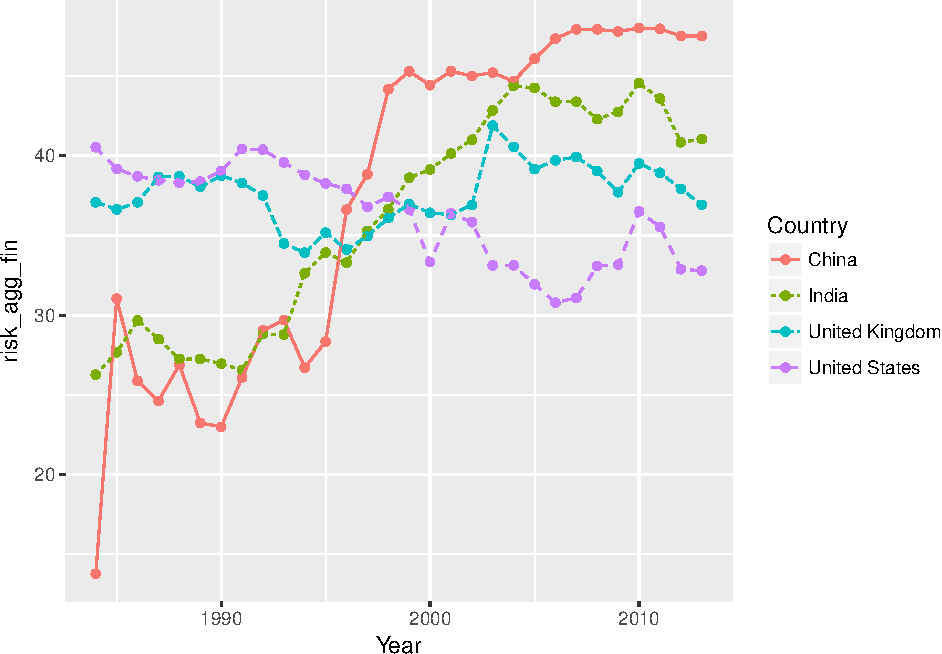
\includegraphics{Intro_read_tidy_files/figure-latex/data_tidy_read-1.pdf}

\subsubsection{Gathering}\label{gathering}

``Gathering'' involves moving column names into a ``key'' column,
gathering the column values into a single value column.

This is used to ``gather'' data from the wide format, to the long
format.

\begin{Shaded}
\begin{Highlighting}[]
\NormalTok{gdppc }\OperatorTok\StringTok{ }\KeywordTok{head}\NormalTok{(.)}
\end{Highlighting}
\end{Shaded}

\begin{verbatim}
## # A tibble: 6 x 61
##   `Series Name`                `Series Code` `Country Name` `Country Code`
##   <chr>                        <chr>         <chr>          <chr>         
## 1 GDP per capita (current US$) NY.GDP.PCAP.~ Afghanistan    AFG           
## 2 GDP per capita (current US$) NY.GDP.PCAP.~ Albania        ALB           
## 3 GDP per capita (current US$) NY.GDP.PCAP.~ Algeria        DZA           
## 4 GDP per capita (current US$) NY.GDP.PCAP.~ American Samoa ASM           
## 5 GDP per capita (current US$) NY.GDP.PCAP.~ Andorra        AND           
## 6 GDP per capita (current US$) NY.GDP.PCAP.~ Angola         AGO           
## # ... with 57 more variables: `1960 [YR1960]` <chr>, `1961
## #   [YR1961]` <chr>, `1962 [YR1962]` <chr>, `1963 [YR1963]` <chr>, `1964
## #   [YR1964]` <chr>, `1965 [YR1965]` <chr>, `1966 [YR1966]` <chr>, `1967
## #   [YR1967]` <chr>, `1968 [YR1968]` <chr>, `1969 [YR1969]` <chr>, `1970
## #   [YR1970]` <chr>, `1971 [YR1971]` <chr>, `1972 [YR1972]` <chr>, `1973
## #   [YR1973]` <chr>, `1974 [YR1974]` <chr>, `1975 [YR1975]` <chr>, `1976
## #   [YR1976]` <chr>, `1977 [YR1977]` <chr>, `1978 [YR1978]` <chr>, `1979
## #   [YR1979]` <chr>, `1980 [YR1980]` <chr>, `1981 [YR1981]` <chr>, `1982
## #   [YR1982]` <chr>, `1983 [YR1983]` <chr>, `1984 [YR1984]` <chr>, `1985
## #   [YR1985]` <chr>, `1986 [YR1986]` <chr>, `1987 [YR1987]` <chr>, `1988
## #   [YR1988]` <chr>, `1989 [YR1989]` <chr>, `1990 [YR1990]` <chr>, `1991
## #   [YR1991]` <chr>, `1992 [YR1992]` <chr>, `1993 [YR1993]` <chr>, `1994
## #   [YR1994]` <chr>, `1995 [YR1995]` <chr>, `1996 [YR1996]` <chr>, `1997
## #   [YR1997]` <chr>, `1998 [YR1998]` <chr>, `1999 [YR1999]` <chr>, `2000
## #   [YR2000]` <chr>, `2001 [YR2001]` <chr>, `2002 [YR2002]` <chr>, `2003
## #   [YR2003]` <chr>, `2004 [YR2004]` <chr>, `2005 [YR2005]` <chr>, `2006
## #   [YR2006]` <chr>, `2007 [YR2007]` <chr>, `2008 [YR2008]` <chr>, `2009
## #   [YR2009]` <chr>, `2010 [YR2010]` <chr>, `2011 [YR2011]` <chr>, `2012
## #   [YR2012]` <chr>, `2013 [YR2013]` <chr>, `2014 [YR2014]` <chr>, `2015
## #   [YR2015]` <chr>, `2016 [YR2016]` <chr>
\end{verbatim}

\begin{Shaded}
\begin{Highlighting}[]
\NormalTok{col_yr_}\DecValTok{1}\NormalTok{ <-}\StringTok{ "1960 [YR1960]"}
\NormalTok{col_yr_end <-}\StringTok{ "2016 [YR2016]"}

\NormalTok{(gdppc_tidy <-}\StringTok{ }\NormalTok{gdppc }\OperatorTok
\StringTok{    }\NormalTok{dplyr}\OperatorTok{::}\KeywordTok{select}\NormalTok{(}\OperatorTok{-}\KeywordTok{c}\NormalTok{(}\StringTok{`}\DataTypeTok{Series Name}\StringTok{`}\NormalTok{, }\CommentTok{#why backticks ``?}
                     \StringTok{`}\DataTypeTok{Series Code}\StringTok{`}\NormalTok{,}
                     \StringTok{`}\DataTypeTok{Country Code}\StringTok{`}
\NormalTok{                     )}
\NormalTok{                  ) }\OperatorTok
\StringTok{    }\NormalTok{dplyr}\OperatorTok{::}\KeywordTok{rename}\NormalTok{(}\DataTypeTok{Country =} \StringTok{`}\DataTypeTok{Country Name}\StringTok{`}\NormalTok{) }\OperatorTok
\StringTok{    }\NormalTok{tidyr}\OperatorTok{::}\KeywordTok{gather}\NormalTok{(col_yr_}\DecValTok{1}\OperatorTok{:}\NormalTok{col_yr_end,}
                  \DataTypeTok{key =} \StringTok{"Year"}\NormalTok{,}
                  \DataTypeTok{value =} \StringTok{"GDP_per_capita"}
\NormalTok{                  ) }\OperatorTok
\StringTok{    }\NormalTok{dplyr}\OperatorTok{::}\KeywordTok{arrange}\NormalTok{(Country)}

\NormalTok{  )}
\end{Highlighting}
\end{Shaded}

\begin{verbatim}
## # A tibble: 15,048 x 3
##    Country     Year          GDP_per_capita
##    <chr>       <chr>         <chr>         
##  1 Afghanistan 1960 [YR1960] 59.7773265084 
##  2 Afghanistan 1961 [YR1961] 59.8781528089 
##  3 Afghanistan 1962 [YR1962] 58.4928738323 
##  4 Afghanistan 1963 [YR1963] 78.7827580363 
##  5 Afghanistan 1964 [YR1964] 82.2084438594 
##  6 Afghanistan 1965 [YR1965] 101.2904712742
##  7 Afghanistan 1966 [YR1966] 137.899361897 
##  8 Afghanistan 1967 [YR1967] 161.3220000885
##  9 Afghanistan 1968 [YR1968] 129.5066538443
## 10 Afghanistan 1969 [YR1969] 129.7985414084
## # ... with 15,038 more rows
\end{verbatim}

\subsubsection{Spreading}\label{spreading}

Spreading is the opposite of gathering. It moves the unique values of a
key column into the column names, thus ``spreading'' the column values
across new columns.

Below, we spread the variable \texttt{fin\_risk} which is in the long
format, into the wide format.

\begin{Shaded}
\begin{Highlighting}[]
\NormalTok{(fin_risk_foreign <-}\StringTok{ }\NormalTok{fin_risk_tidy }\OperatorTok\StringTok{ }
\StringTok{  }\NormalTok{dplyr}\OperatorTok{::}\KeywordTok{select}\NormalTok{(}\KeywordTok{c}\NormalTok{(Country, Year, risk_foreign))}
\NormalTok{ )}
\end{Highlighting}
\end{Shaded}

\begin{verbatim}
## # A tibble: 4,380 x 3
##    Country  Year risk_foreign
##    <chr>   <int>        <dbl>
##  1 Albania  1984         5.33
##  2 Albania  1985         6   
##  3 Albania  1986         6   
##  4 Albania  1987         6   
##  5 Albania  1988         6.25
##  6 Albania  1989         6.54
##  7 Albania  1990         6.96
##  8 Albania  1991         6.75
##  9 Albania  1992         4.58
## 10 Albania  1993         4   
## # ... with 4,370 more rows
\end{verbatim}

\begin{Shaded}
\begin{Highlighting}[]
\NormalTok{(fin_risk_spread <-}\StringTok{ }\NormalTok{fin_risk_foreign }\OperatorTok
\StringTok{  }\NormalTok{tidyr}\OperatorTok{::}\KeywordTok{spread}\NormalTok{(}\DataTypeTok{key =}\NormalTok{ Country, }
                \DataTypeTok{value =}\NormalTok{ risk_foreign}
\NormalTok{                )}
\NormalTok{  )}
\end{Highlighting}
\end{Shaded}

\begin{verbatim}
## # A tibble: 30 x 147
##     Year Albania Algeria Angola Argentina Armenia Australia Austria
##    <int>   <dbl>   <dbl>  <dbl>     <dbl>   <dbl>     <dbl>   <dbl>
##  1  1984    5.33    5.55   4         1.8       NA      8.52    8.55
##  2  1985    6       6      4         1.54      NA      8.33    8.5 
##  3  1986    6       4.83   2.83      2         NA      7.75    8.13
##  4  1987    6       4.29   2.75      2.92      NA      7.5     8.42
##  5  1988    6.25    4.58   3         3.33      NA      8       9   
##  6  1989    6.54    5.5    3.08      3.54      NA      8.5     9   
##  7  1990    6.96    6.25   3         2.42      NA      8.96    9   
##  8  1991    6.75    7.13   3         4.79      NA      9       9   
##  9  1992    4.58    5.96   3.46      6.96      NA      8.88    9.71
## 10  1993    4       4.5    2.79      6.38      NA      8       9.5 
## # ... with 20 more rows, and 139 more variables: Azerbaijan <dbl>,
## #   Bahamas <dbl>, Bahrain <dbl>, Bangladesh <dbl>, Belarus <dbl>,
## #   Belgium <dbl>, Bolivia <dbl>, Botswana <dbl>, Brazil <dbl>,
## #   Brunei <dbl>, Bulgaria <dbl>, `Burkina Faso` <dbl>, Cameroon <dbl>,
## #   Canada <dbl>, Chile <dbl>, China <dbl>, Colombia <dbl>, Congo <dbl>,
## #   `Congo, DR` <dbl>, `Costa Rica` <dbl>, `Cote d'Ivoire` <dbl>,
## #   Croatia <dbl>, Cuba <dbl>, Cyprus <dbl>, Czechoslovakia <dbl>, `Czech
## #   Republic` <dbl>, Denmark <dbl>, `Dominican Republic` <dbl>, `East
## #   Germany` <dbl>, Ecuador <dbl>, Egypt <dbl>, `El Salvador` <dbl>,
## #   Estonia <dbl>, Ethiopia <dbl>, Finland <dbl>, France <dbl>,
## #   Gabon <dbl>, Gambia <dbl>, Germany <dbl>, Ghana <dbl>, Greece <dbl>,
## #   Guatemala <dbl>, Guinea <dbl>, `Guinea Bissau` <dbl>, Guyana <dbl>,
## #   Haiti <dbl>, Honduras <dbl>, `Hong Kong` <dbl>, Hungary <dbl>,
## #   Iceland <dbl>, India <dbl>, Indonesia <dbl>, Iran <dbl>, Iraq <dbl>,
## #   Ireland <dbl>, Israel <dbl>, Italy <dbl>, Jamaica <dbl>, Japan <dbl>,
## #   Jordan <dbl>, Kazakhstan <dbl>, Kenya <dbl>, `Korea, DPR` <dbl>,
## #   Kuwait <dbl>, Latvia <dbl>, Lebanon <dbl>, Liberia <dbl>, Libya <dbl>,
## #   Lithuania <dbl>, Luxembourg <dbl>, Madagascar <dbl>, Malawi <dbl>,
## #   Malaysia <dbl>, Mali <dbl>, Malta <dbl>, Mexico <dbl>, Moldova <dbl>,
## #   Mongolia <dbl>, Morocco <dbl>, Mozambique <dbl>, Myanmar <dbl>,
## #   Namibia <dbl>, Netherlands <dbl>, `New Caledonia` <dbl>, `New
## #   Zealand` <dbl>, Nicaragua <dbl>, Niger <dbl>, Nigeria <dbl>,
## #   Norway <dbl>, Oman <dbl>, Pakistan <dbl>, Panama <dbl>, `Papua New
## #   Guinea` <dbl>, Paraguay <dbl>, Peru <dbl>, Philippines <dbl>,
## #   Poland <dbl>, Portugal <dbl>, Qatar <dbl>, Romania <dbl>, ...
\end{verbatim}

Each column now is the aggregate foreign financial risk of a country.
This is the wide format.

\subsubsection{Joining}\label{joining}

\texttt{fin\_risk\_foreign} and \texttt{gdppc\_tidy} are both tidy
datasets containing information about countries' foreign financial risk
variables and GDP per capita respectively. What if we wish to merge the
two datasets into one, so that we have countries' risk as well as GDP
per capita profiles?

This can be achieved by the so-called ``mutating join'' family of
functions from \texttt{dplyr}. There are mainly four types of joins:

\begin{enumerate}
\def\labelenumi{\arabic{enumi}.}
\tightlist
\item
  \texttt{left\_join(x,\ y)} merges \texttt{y} using matching values for
  \texttt{x}.
\item
  \texttt{right\_join(x,\ y)} merges \texttt{x} using matching values
  for \texttt{y}.
\item
  \texttt{inner\_join(x,\ y)} merges only matching rows.
\item
  \texttt{full\_join(x,\ y)} merges fully, retaining all values.
\end{enumerate}

Missing matches are filled with \texttt{NA} values.

\begin{Shaded}
\begin{Highlighting}[]
\NormalTok{gdppc_tidy}\OperatorTok{$}\NormalTok{Year <-}\StringTok{ }\DecValTok{1960}\OperatorTok{:}\DecValTok{2016} \CommentTok{#reformatting dates}

\CommentTok{# Left Joining}
\NormalTok{(data_join_left <-}\StringTok{ }\NormalTok{dplyr}\OperatorTok{::}\KeywordTok{left_join}\NormalTok{(fin_risk_foreign, gdppc_tidy, }
                                   \DataTypeTok{by =} \KeywordTok{c}\NormalTok{(}\StringTok{"Country"}\NormalTok{, }\StringTok{"Year"}\NormalTok{)}
\NormalTok{                                   ) }\OperatorTok
\StringTok{    }\NormalTok{dplyr}\OperatorTok{::}\KeywordTok{arrange}\NormalTok{(Country)}
\NormalTok{  )}
\end{Highlighting}
\end{Shaded}

\begin{verbatim}
## # A tibble: 4,380 x 4
##    Country  Year risk_foreign GDP_per_capita
##    <chr>   <int>        <dbl> <chr>         
##  1 Albania  1984         5.33 662.5200523091
##  2 Albania  1985         6    662.9147925671
##  3 Albania  1986         6    719.1572957039
##  4 Albania  1987         6    699.3842920867
##  5 Albania  1988         6.25 676.56673252  
##  6 Albania  1989         6.54 723.4096102379
##  7 Albania  1990         6.96 639.4638992899
##  8 Albania  1991         6.75 348.711317787 
##  9 Albania  1992         4.58 218.4921659026
## 10 Albania  1993         4    380.5273710843
## # ... with 4,370 more rows
\end{verbatim}

\begin{Shaded}
\begin{Highlighting}[]
\CommentTok{# Right Joining}
\NormalTok{(data_join_right <-}\StringTok{ }\NormalTok{dplyr}\OperatorTok{::}\KeywordTok{right_join}\NormalTok{(fin_risk_foreign, gdppc_tidy, }
                                   \DataTypeTok{by =} \KeywordTok{c}\NormalTok{(}\StringTok{"Country"}\NormalTok{, }\StringTok{"Year"}\NormalTok{)}
\NormalTok{                                   ) }\OperatorTok
\StringTok{    }\NormalTok{dplyr}\OperatorTok{::}\KeywordTok{arrange}\NormalTok{(Country)}
\NormalTok{  )}
\end{Highlighting}
\end{Shaded}

\begin{verbatim}
## # A tibble: 15,048 x 4
##    Country      Year risk_foreign GDP_per_capita
##    <chr>       <int>        <dbl> <chr>         
##  1 Afghanistan  1960           NA 59.7773265084 
##  2 Afghanistan  1961           NA 59.8781528089 
##  3 Afghanistan  1962           NA 58.4928738323 
##  4 Afghanistan  1963           NA 78.7827580363 
##  5 Afghanistan  1964           NA 82.2084438594 
##  6 Afghanistan  1965           NA 101.2904712742
##  7 Afghanistan  1966           NA 137.899361897 
##  8 Afghanistan  1967           NA 161.3220000885
##  9 Afghanistan  1968           NA 129.5066538443
## 10 Afghanistan  1969           NA 129.7985414084
## # ... with 15,038 more rows
\end{verbatim}

\begin{Shaded}
\begin{Highlighting}[]
\CommentTok{# Inner Joining}
\NormalTok{(data_join_inner <-}\StringTok{ }\NormalTok{dplyr}\OperatorTok{::}\KeywordTok{inner_join}\NormalTok{(fin_risk_foreign, gdppc_tidy, }
                                   \DataTypeTok{by =} \KeywordTok{c}\NormalTok{(}\StringTok{"Country"}\NormalTok{, }\StringTok{"Year"}\NormalTok{)}
\NormalTok{                                   ) }\OperatorTok
\StringTok{    }\NormalTok{dplyr}\OperatorTok{::}\KeywordTok{arrange}\NormalTok{(Country)}
\NormalTok{  )}
\end{Highlighting}
\end{Shaded}

\begin{verbatim}
## # A tibble: 3,660 x 4
##    Country  Year risk_foreign GDP_per_capita
##    <chr>   <int>        <dbl> <chr>         
##  1 Albania  1984         5.33 662.5200523091
##  2 Albania  1985         6    662.9147925671
##  3 Albania  1986         6    719.1572957039
##  4 Albania  1987         6    699.3842920867
##  5 Albania  1988         6.25 676.56673252  
##  6 Albania  1989         6.54 723.4096102379
##  7 Albania  1990         6.96 639.4638992899
##  8 Albania  1991         6.75 348.711317787 
##  9 Albania  1992         4.58 218.4921659026
## 10 Albania  1993         4    380.5273710843
## # ... with 3,650 more rows
\end{verbatim}

\begin{Shaded}
\begin{Highlighting}[]
\CommentTok{# Full Joining}
\NormalTok{(data_join_full <-}\StringTok{ }\NormalTok{dplyr}\OperatorTok{::}\KeywordTok{full_join}\NormalTok{(fin_risk_foreign, gdppc_tidy, }
                                   \DataTypeTok{by =} \KeywordTok{c}\NormalTok{(}\StringTok{"Year"}\NormalTok{, }\StringTok{"Country"}\NormalTok{)}
\NormalTok{                                   ) }\OperatorTok
\StringTok{    }\NormalTok{dplyr}\OperatorTok{::}\KeywordTok{arrange}\NormalTok{(Country)}
\NormalTok{  )}
\end{Highlighting}
\end{Shaded}

\begin{verbatim}
## # A tibble: 15,768 x 4
##    Country      Year risk_foreign GDP_per_capita
##    <chr>       <int>        <dbl> <chr>         
##  1 Afghanistan  1960           NA 59.7773265084 
##  2 Afghanistan  1961           NA 59.8781528089 
##  3 Afghanistan  1962           NA 58.4928738323 
##  4 Afghanistan  1963           NA 78.7827580363 
##  5 Afghanistan  1964           NA 82.2084438594 
##  6 Afghanistan  1965           NA 101.2904712742
##  7 Afghanistan  1966           NA 137.899361897 
##  8 Afghanistan  1967           NA 161.3220000885
##  9 Afghanistan  1968           NA 129.5066538443
## 10 Afghanistan  1969           NA 129.7985414084
## # ... with 15,758 more rows
\end{verbatim}


\end{document}
